\chapter[Projekt rękawicy]{Projekt rękawicy\raisebox{.3\baselineskip}{\normalsize\footnotemark}}
\footnotetext{Poniższy rozdział jest częścią pracy inżynierskiej, wykorzystującej zbudowany kontroler jako bazę dla aplikacji pracującej na pozyskanych danych~\cite{H}.}
\label{ch:projekt}
Istotą poniższego rozdziału jest pokazanie użytych w projekcie podzespołów i technologii oraz lepsze zrozumienie powodów dla których to właśnie te produkty zostały wybrane. Po zapoznaniu się z motywem, zostanie szczegółowo opisana specyfikacja tych produktów a także sposób ich poskładania w spójną całość. Po nakreśleniu podstawowych założeń projektu zostanie zaprezentowana finałowa wersja, a także szczegółowo zostanie omówiony kod rękawicy-kontrolera, który jest obsługiwany przez mikrokontroler. Kluczowym dla powodzenia projektu jest ustalenie podstawowych informacji uzyskiwanych z kontrolera takich jak orientacja dłoni względem punktu początkowego oraz moment i stopień zgięcia palców. W tym celu należy zebrać informacje z czujników, a następnie wszystkie te informacje należy przesłać do pożądanego urządzenia. Elementem które pozwala to osiągnąć w tym projekcie jest mikrokontroler Arduino nano 33 BLE, który odpowiada za dostarczenie informacji z żyroskopu, akcelerometru a także czujników wygięcia. W poniższych sekcjach zostanie opisane rozwiązanie zastosowane do pozyskania danych z tych czujników, odczytu położenia palców, zasada działania przy wykorzystaniu rezystorów oraz sposób połączenia wszystkich wspomnianych elementów w finałową wersję kontrolera.
	
	
	\section{Mikrokontroler}
	\label{sec:arduino}
	Jak przed chwilą wspomniano, w projekcie wykorzystywana jest płytka od Arduino, która nosi nazwę Nano 33 BLE. Jest to małych rozmiarów płytka o  wymiarach 45 x 18 mm, pozwalająca na wysoką wydajność przy jednoczesnym małym poborze prądu, co zapewnia użyty mikrokontroler nRF52480 o taktowaniu 64 MHz. Do dyspozycji mamy również pamięć RAM o pojemności 256 kB oraz pamięć Flash o pojemności 1 MB. IMU które zostało zamontowane na płytce to LSM9DS1, które obsługuję akcelerometr, żyroskop oraz magnetometr w trzech osiach. Pozwala to na określenie rotacji w aplikacji obsługującej kontroler bazując na odczytach żyroskopu. Akcelerometr nie jest wystarczająco dokładny aby móc określić położenie w przestrzeni z powodu generowanych błędów, które z czasem sprawiają że odczyty są bezużyteczne. Aby określić położenie kontrolera w przestrzeni należy zastosować zewnętrzny system śledzenia, którego ze względu na prostotę oraz uniwersalność projektu nie zastosowano~\cite{displacement}. Warto na wstępie zauważyć że Nano 33 BLE pracuje domyślnie wyłącznie z napięciem 3,3 V, w związku z czym nie należy podłączać bezpośrednio zasilania o większym napięciu. W celu podłączenia zasilania 5 V należy zlutować zworkę znajdującą się pomiędzy pinami RDT oraz A7. Płytka ta posiada wiele użytecznych sensorów, jednak na potrzeby tej pracy została wybrana z powodu wbudowanej inercyjnej jednostki pomiarowej, dzięki czemu można było uprościć konstrukcję oraz zmniejszyć ilość połączeń na rękawicy, wbudowanego modułu Bluetooth - a w tym przypadku modułu Bluetooth Low Energy obsługiwanego w standardzie 5.0, a to wszystko w przystępnej cenie co również było jednym z kryteriów przy tworzeniu tego projektu. Płytkę w momencie tworzenia tej pracy można kupić za 119 zł. Wartym uwagi jest fakt możliwości zakupu płytki bez wyprowadzonych złącz, co w przypadku opisywanego projektu pozwoli na zmniejszenie wymiarów oraz większą swobodę montażu~\cite{botland-arduino}.
\begin{figure}[h]
\centering
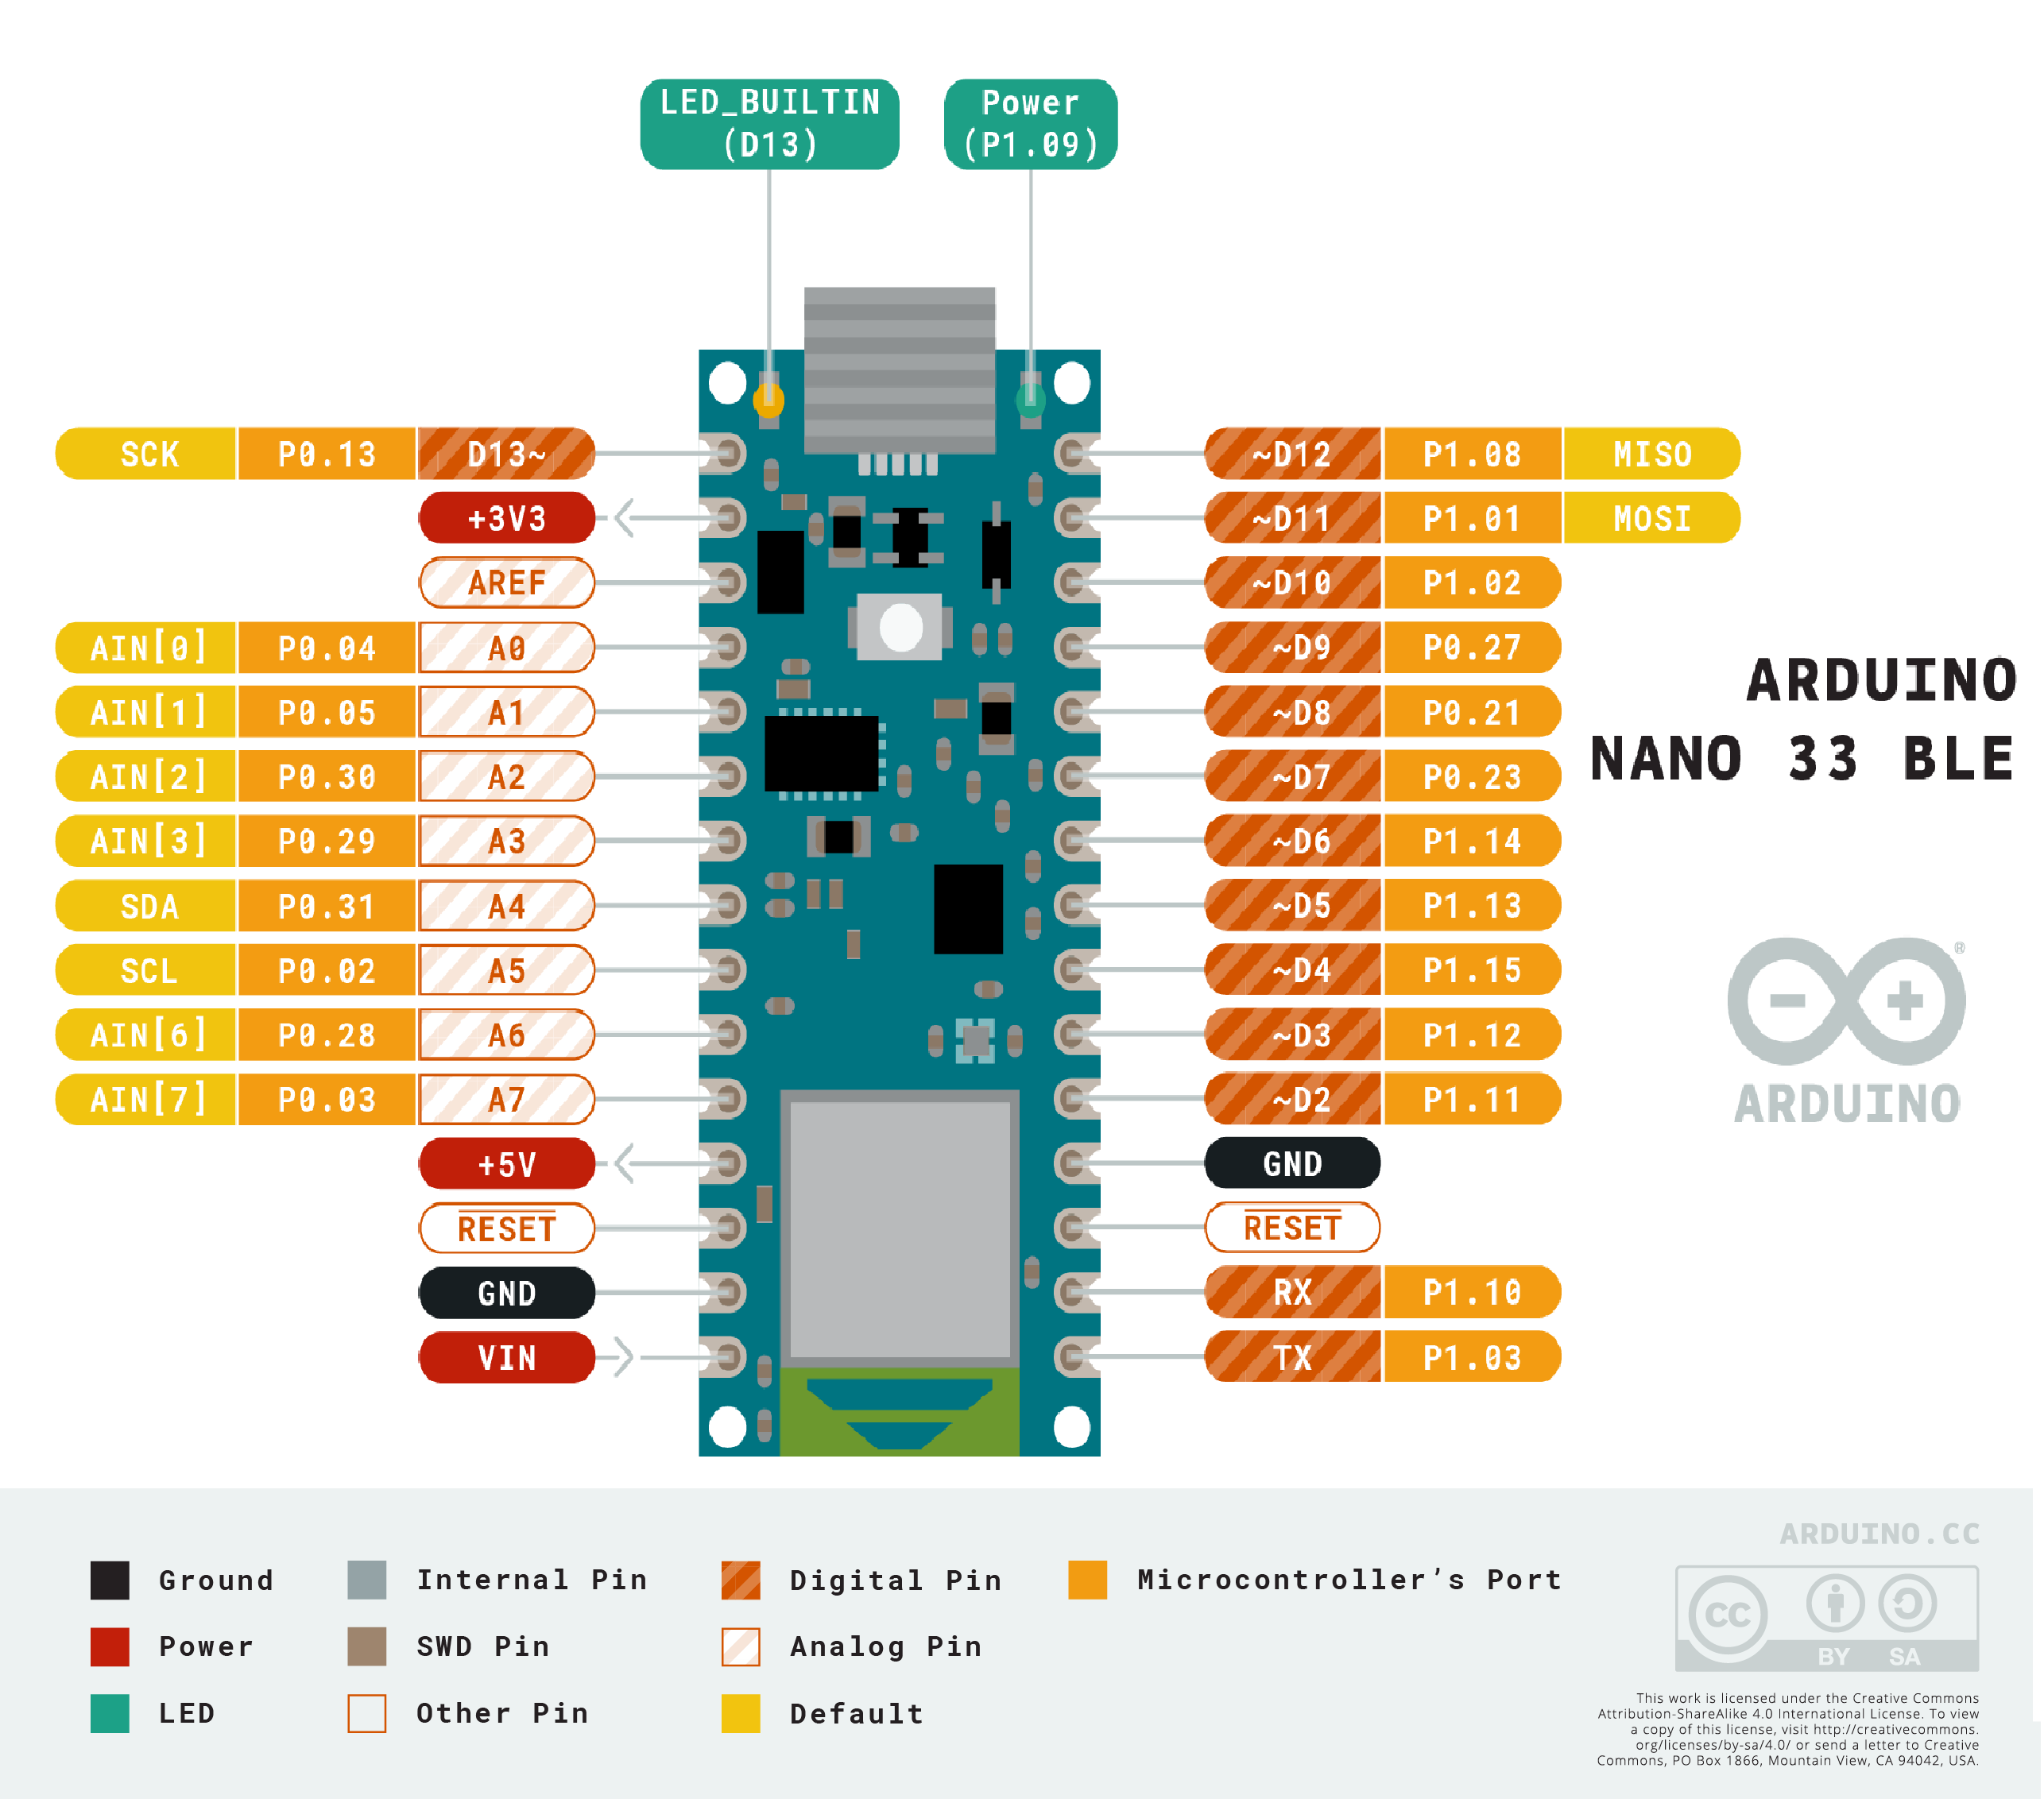
\includegraphics[scale=0.5]{arduino}
\captionsource{Opis wejść oraz wyjść Arduino Nano 33 BLE}{\url{https://content.arduino.cc/assets/Pinout-NANOble_latest.pdf}}
\label{fig:arduino}
\end{figure}
	
	Z najważniejszych elementów układu płytki należy wiedzieć że posiada ona dwa piny wyjściowe zasilające o napięciu 3,3 V oraz 5 V, jeden pin zasilający wejściowy, a także dwa piny uziemiające, po jednym z każdej strony płytki. Posiada ona piny zarówno analogowe jak i cyfrowe, jednak na potrzeby tego projektu zostały użyte jedynie piny analogowe, których do dyspozycji jest osiem, umiejscowionych po jednej stronie, przy czym warto zwrócić uwagę że piny A4 oraz A5 używane są jako magistrala I2C w związku z czym zalecane jest nie stosowanie tych wejść analogowych. Szczegółowy opis wejść/wyjść płytki przedstawiony jest na grafice~\ref{fig:arduino}. W tym projekcie wykorzystano zasilanie poprzez złącze micro USB, wyjście o napięciu 3,3 V w celu uzyskania odczytów z czujników wygięcia na pinach analogowych A0, A1, A3, A6 oraz A7, o których zostanie więcej powiedziane w punkcie~\ref{sec:budowa}, a także uziemienie znajdujące się po tej samej stronie płytki.

	\section{Czujnik wygięcia}
	\label{sec:wygiecie}	
	Kluczowym dla działania kontrolera jest możliwość określenia pozycji palców względem dłoni. Ma to wiele zastosowań zarówno wizualnych jak i praktycznych. Ważne jest aby odwzorować świat rzeczywisty tak dokładnie jak to możliwe - im lepsze odwzorowanie tym bardziej zmysły użytkownika zostaną oszukane, podwyższając komfort użytkowania technologii wirtualnej rzeczywistości. Za stroną praktyczną natomiast przemawia możliwość śledzenia palców w celu dokładnego ich użycia w stworzonym środowisku np. do ściskania i podnoszenia obiektów czy też korzystania z klawiatury wirtualnej. Wśród znanych producentów na rynku, decyduję się oni na użycie wielu inercyjnych jednostek pomiarowych, na podstawie których są w stanie dokładnie określić położenia każdej części palca, bądź też nie aż tak popularne rozwiązanie, które wykorzystujące specjalistyczne sensory służące do pomiaru stopnia wygięcia czujnika względem pozycji prostej. Czujnik ten po podłączeniu do prądu zwiększa swój opór wraz ze zwiększonym stopniem odchylenia. Oba te rozwiązania pomimo wysokiej dokładności pomiarów nie są rozwiązaniami tanimi. W związku z tym na potrzeby stworzenia taniego kontrolera, należało znaleźć rozwiązanie bardziej przystępna a jednocześnie pozwalające na osiągnięcie tego samego celu.
	
	Aby osiągnąć postawione założenia zostały skonstruowane czujniki wygięcia w domowych warunkach. Rozwiązanie to jest często używane do osiągnięcia pomiaru stopnia wygięcia bez konieczności wydawania ponad 100 zł na jeden czujnik~\cite{flex-sensor}. Jest ono stosunkowo proste w założeniach i wymaga jedynie dwóch kluczowych elementów. Tkaniny przewodzącej o specjalnych właściwościach oraz dwóch przewodników po obu stronach materiału. Z jednej strony zostanie podłączone napięcie z drugiej natomiast uziemienie. Ważnym jest aby połączenia te się ze sobą nie stykały w żadnym punkcie a jedynie zostały nałożone na siebie, z tkaniną ściśniętą pomiędzy nimi - dzięki temu mamy pewność że odczyty które otrzymamy będą prawidłowe. Pozostaje odpowiedzieć na pytanie jakiego rodzaju materiał należy wykorzystać. Na rynku znajdziemy wiele rodzajów materiałów które zmieniają swój opór w zależności od spełnienia takich kryteriów jak nacisk, temperatura, rozciągnięcie czy też właśnie zgięcie materiału. Zdecydowano się na użycie foli Velostat która jest czuła na nacisk or zginanie~\cite{velostat}. W roli przewodnika wybrano nić przewodzącą, która zapewniła potrzebną elastyczność oraz możliwość przymocowania poszczególnych elementów przy jednoczesnym zapewnieniu funkcjonalności. Elementy te zostały sklejone na kawałku taśmy samoprzylepnej oraz dodatkowo sklejone przy brzegu aby nić nie wyśliznęła się w trakcie korzystania z czujnika. Efekt końcowy jest widoczny na zdjęciu~\ref{fig:sensor}. W celu otrzymania pomiarów wszystkich palców zostało wykonanych pięć takich sensorów, o szerokości 15 mm; dwa o długości 8 cm, dwa o długości 10 cm a także jeden 11 cm, w celu jak najlepszego dopasowania względem miejsca na palce na zakupionej rękawicy do której sensory zostaną przymocowane, co można zobaczyć na zdjęciu~\ref{fig:glove}.
	
\begin{figure}[h]
\centering
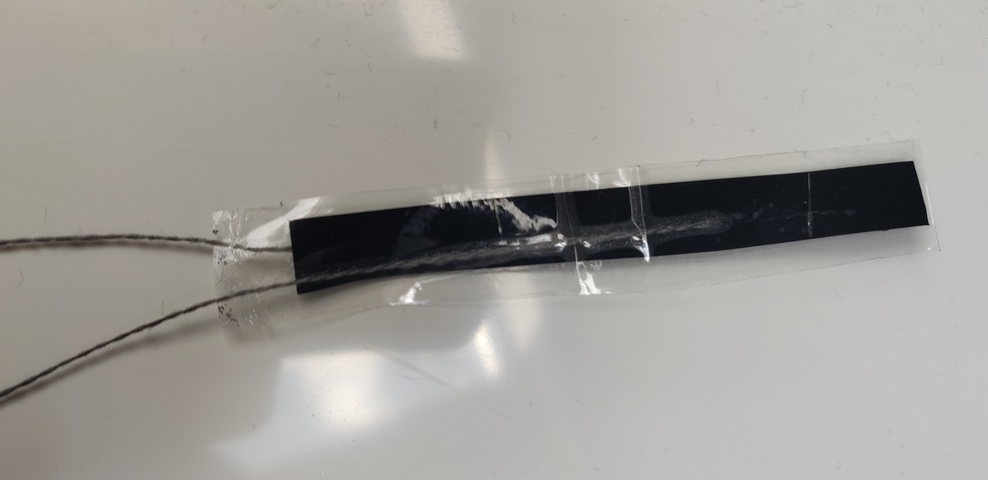
\includegraphics[scale=0.65,width=\textwidth]{flex-sensor}
\caption{Sensor wygięcia własnego wykonania}
\label{fig:sensor}
\end{figure}	

	\section{Rezystor}
	\label{sec:rezystor}	
	Rezystor, potocznie zwany opornikiem, jest to prosty element elektroniczny, posiadający jedynie wyjścia z dwóch stron elementu łączącego. Element ten tworzy opór, powodując ograniczenie przepływającego przez niego prądu gdy jest włączony do obwodu szeregowo. Opór ten jest mierzony w omach. Istotną informacją jest fakt że nadmiar prądu jest zamieniany przez opornik na energie cieplną, a także brak zdefiniowanego kierunku - co oznacza że działa on niezależnie od sposoby zanotowania go w układzie.
	
	Podstawową wartością na którą należy zwrócić uwagę jest rezystancja. Rezystancję podaje się w omach i można spotkać na rynku zakres od miliomów do megaomów. Spośród dostępnych rodzajów rezystorów w projekcie zostały użyte rezystory THT ( z ang. Through-Hole Technology) - czyli tak zwane rezystory do montażu przewlekanego. W tym rodzaju oporników rezystancja jest ilustrowana poprzez kolorowe paski umieszczone wokół oporu, co pozwala odczytać ich wartość według ilustracji~\ref{fig:oporniki}. Alternatywą do tego sposobu jest podłączenie rezystora pod miernik elektryczny ustawiony w tryb pomiaru oporu~\cite{rezystor}. Element ten jest kluczowy w celu ograniczenia przepływu prądu w obwodzie rękawicy, co pozwala na monitorowanie oporu wytwarzanego poprzez czujnik wygięcia.
		
\begin{figure}[h]
\centering
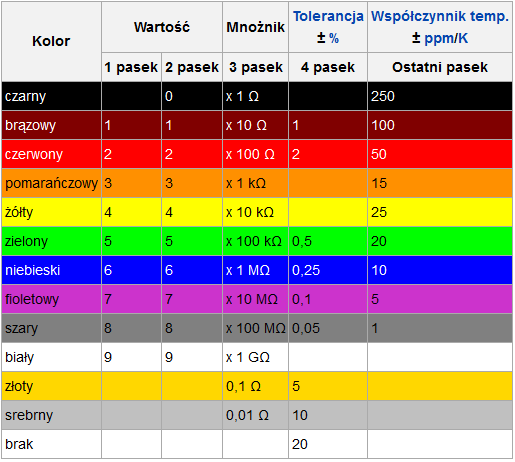
\includegraphics[scale=0.65]{oporniki}
\captionsource{Oznaczenia rezystorów}{\url{https://sites.google.com/site/informatykaunijna/home/poszczegolne-czesci/rezystor}}
\label{fig:oporniki}
\end{figure}
	
Sposób działania układu, nazywanego dzielnikiem napięcia, wyraża się wzorem
	$
		\nu_{out} = \nu_{in}\left[ \frac{R_2}{R_1+R_2}\right]
	$	
Wzór ten podaje napięcie wyjściowe $\nu_{out}$, które równa się napięciu wejściowemu $\nu_{in}$ przeskalowanemu przez stosunek rezystorów. W opisywanym przypadku jest to stosunek zastosowanego rezystora $4.7 k\Omega$ wyrażonego we wzorze poprzez $R_2$, do sumy tego rezystora wraz z oporem wytwarzanym poprzez czujnik wygięcia $R_1$, który jest zmienny. Oznacza to że im bardziej czujnik wygięcia jest zgięty, wytwarza on większy opór a co za tym idzie napięcie wyjściowe spada. Miara ta obrazuje jak bardzo palec jest zgięty i jest możliwa do uzyskania właśnie dzięki zastosowaniu układu dzielnika napięcia~\cite{v-divider}.


\section{Budowa rękawicy}
\label{sec:budowa}

W poniższej sekcji zaprezentowano sposób w jaki zostały złączone wszystkie elementy rękawicy, aby była gotowa na oprogramowanie mikrokontrolera tworząc finałowy produkt. Jak wspomniano w sekcji~\ref{sec:wygiecie}, do połączenia elementów została wykorzystana nić przewodząca. Dzięki grubym włóknom rękawicy, odstępy pomiędzy nićmi przewodzącymi prąd mogły być mniejsze, bez obawy przed spięciami w trakcie poruszania ręką. Dla tego projektu kontroler jest budowany dla lewej dłoni.

\begin{figure}[h]
\centering
%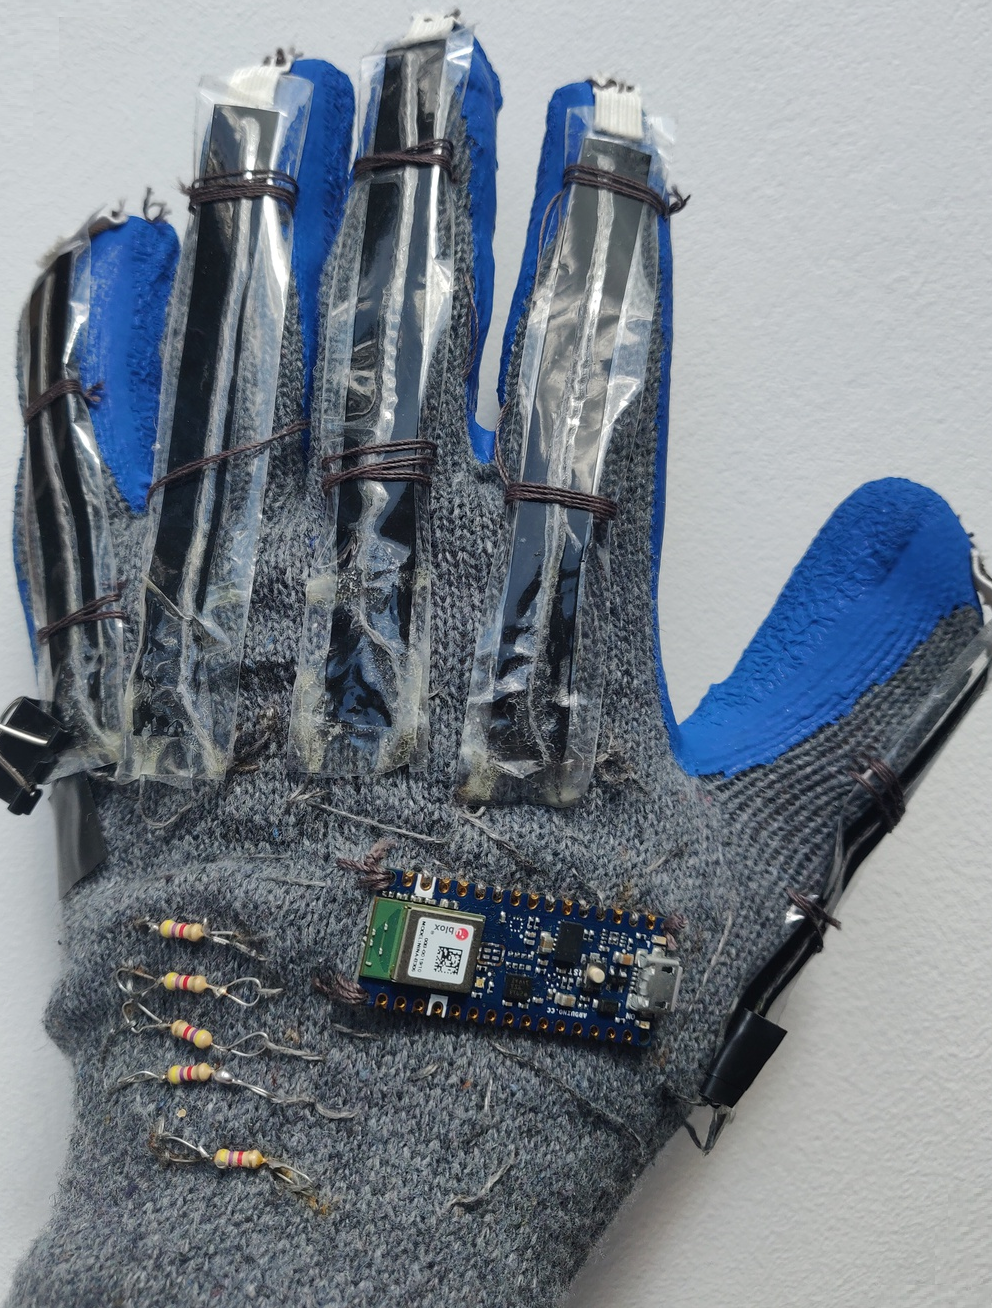
\includegraphics[width=\textwidth]{glove}
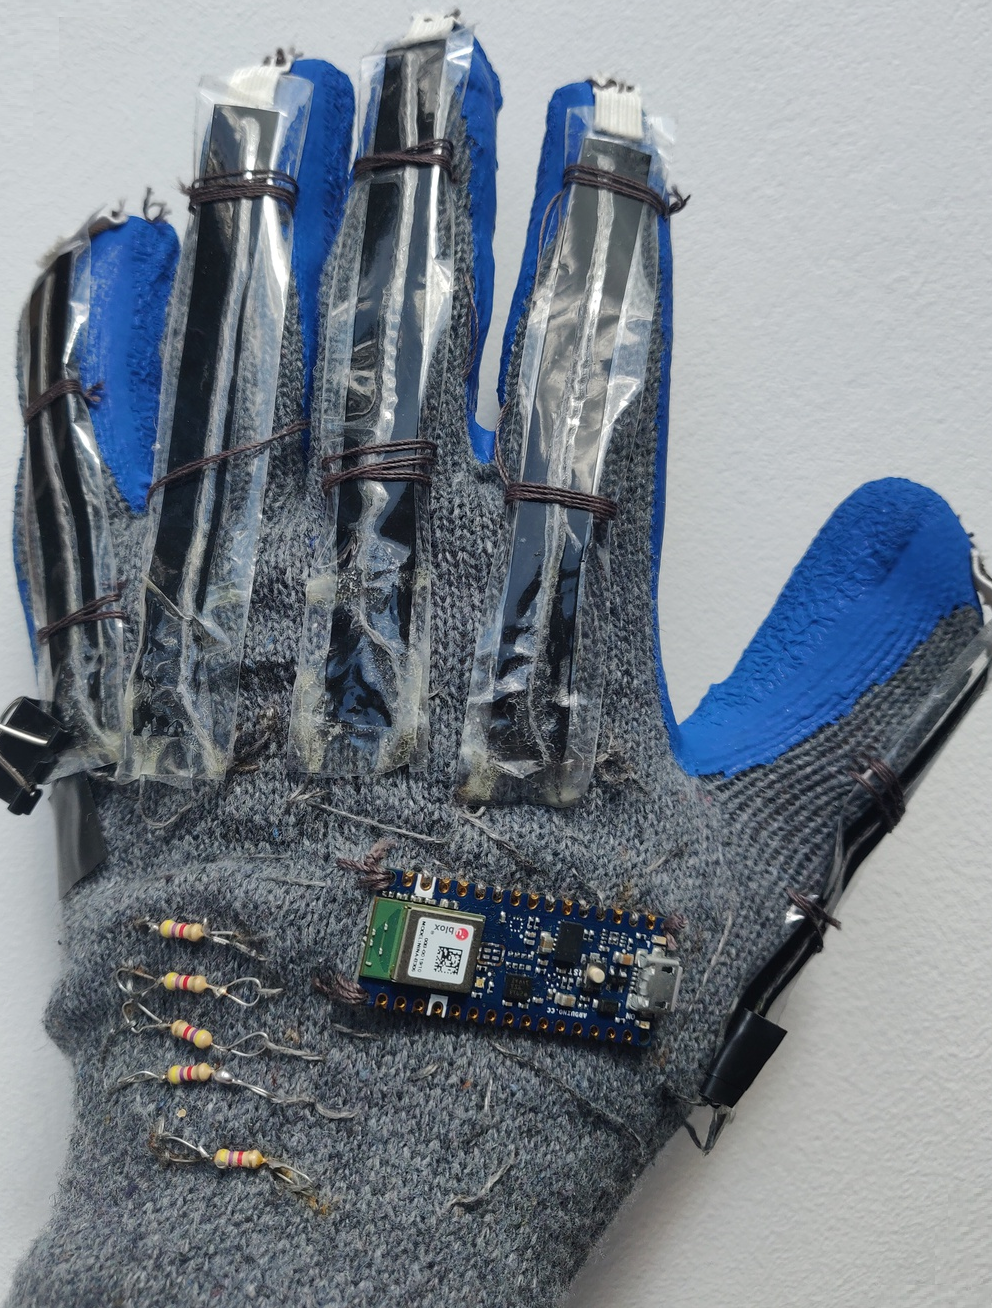
\includegraphics[scale = 0.35]{glove}
\caption{Efekt końcowy rękawicy-kontrolera}
\label{fig:glove}
\end{figure}

Mikroprocesor został umieszczony na wysokości centralnej części dłoni, przy kciuku, skierowany złączem USB na zewnątrz, pozwalając na łatwe podłączenie przewodu zasilającego jak i również ustawienie wejść analogowych w stronę palców lewej dłoni. Z tej strony płytki Arduino będziemy też korzystać - zarówno przy wyprowadzaniu napięcia jak i uziemienia. Montaż samej płytki nie stanowi żadnego problemu ze względy na cztery otwory w rogach pozwalające na mocowanie, do którego została użyta zwykła nić do szycia. Aby stworzyć obwód wychodzący od pinu GND (z ang. Ground) czyli właśnie uziemienia, należy najpierw poprowadzić go przez rezystory. W tym celu wyjścia oporników zostały wygięte w pętle oraz zalutowane aby w łatwy sposób można było je przyszyć do rękawicy. Aby dodatkowo ułatwić sobie to zadanie - dodatkowo zostały one przyklejone bezpośrednio do materiału na kroplę kleju. Umiejscowienie rezystorów jest po zewnętrznej wierzchniej stronie dłoni, zaczynając się na wysokości kontrolera, zmierzając szeregowo w stronę nadgarstka. W ten oto sposób nić przewodząca została poprowadzona na zewnętrzną część dłoni a następnie poprzez wszystkie pętle rezystorów, kończąc na ostatnim. Z drugiej strony rezystora dochodzi natomiast nić pochodząca z czujnika oporu. W tym celu podczas tworzenia czujników oporu pozostawiono 25 cm długości nici, co pozwoliło na przymocowanie sensorów, a następnie połączenie obwodu. Sensory zostały zaopatrzone w krótkie, 1-2 cm długości kawałki taśmy elastycznej która została przyklejona na czubku każdego z sensorów pozwalając na elastyczny ruch sensora bez zerwania nici. Taśma ta została przyszyta w czubkach palców co dało punkt zaczepu dla sensorów. W tym momencie pozwoliło to na wygodne używanie nici wychodzących z sensorów w celu zamknięcia obwodu. Z powodu dużego zagęszczenia nici, które nie mogą się ze sobą stykać podczas ruchu ręki, ważnym dla projektu było naprzemienne używanie przestrzeni na rękawicy od spodu jak i od góry. Dzięki temu nici uziemienia oraz napięcia mogą się krzyżować nie zaburzając przy tym odczytów z sensorów. W celu jak najlepszego zagospodarowania przestrzenią wokół sensorów, uziemienie kciuka oraz małego palca zostały umiejscowione na nicie wychodzącej z prawej strony sensora, natomiast napięcie po lewej stronie. Dla pozostałych palców ustawienie to jest odwrotne. Mając to na uwadze została poprowadzona nić od kciuka poprzez wyjście 3.3 V na płytce a następnie wzdłuż knykci rękawicy, pozwalając nicią odpowiedzialnym za napięcie w odpowiednich sensorach na przyczepienie się w celu poboru napięcia tworząc tym samym dodatnią stronę układu. Nici wychodzące z sensorów które natomiast nie zostały do tej pory użyte, zostały przeszyte poprzez wyjścia analogowe a następnie podłączone kolejno do odpowiadających im rezystorów. Wyjścia odpowiadające każdemu z palców zostały opisane w tabeli poniżej. 

\begin{center}
\begin{tabular}{|c|c|}
\hline
Palec & Wyjście analogowe \\ \hline
Kciuk & A3 \\ \hline
Wskazujący & A0 \\ \hline
Środkowy & A1 \\ \hline
Serdeczny & A6 \\ \hline
Mały & A7 \\ \hline
\hline
\end{tabular}
\end{center}

Sposób w jaki zostały dobrane wyjścia jest podyktowany zaleceniami o nie korzystaniu z wyjść analogowych A4 oraz A5 oraz pozostawieniu przestrzeni wokół wyjścia A3 przeznaczonego na kciuka, ponieważ jako jedyne połączenie musiało najpierw zmierzać w kierunku palców a następnie w dół w celu połączenia z rezystorem. Efekt końcowy pracy przedstawia zdjęcie~\ref{fig:glove}.

\section{Oprogramowanie mikrokontrolera}
\label{sec:oprogramowanie}

W niniejszej sekcji przedstawiony jest kod programu który został napisany w środowisku programistycznym oraz języku o tej samej nazwie - Arduino. Język ten poza drobnymi zmianami opiera się na języku C/C++, a jego pełny kod źródłowy jest dostępny na platformie Github~\cite{jArduino}. Aby rozpocząć pracę z wybranym produktem od Arduino należy wykonać pewne czynności przygotowywacze, takie jak instalacja sterowników płytki dla danego systemu czy sposób obsługi w samym środowisku Arduino. Czynności te zostały opisane na stronie producenta, w związku z czym nie zostaną one szczegółowo opisane~\cite{guideArduino}. Po spełnieniu wszystkich wymagań, został przygotowany program który został napisany oraz wgrany do mikrokontrolera, który można podzielić na trzy części: deklaracje, ustawienie mikrokotrnolera, główna pętla programu.

W pierwszej kolejności zostanie przedstawiona część deklaracji, w której to dołączono wymagane biblioteki dla poprawnej obsługi wszystkich sensorów. Pierwszą biblioteką która została dołączona do programu jest \textit{Arduino\textunderscore LSM9DS1.h}. Biblioteka ta jest odpowiedzialna za obsługę IMU która przekazuje dane poprzez I2C do mikroprocesora. Biblioteka ta zajmuję się obsługą połączenia jak i kalibracja całego modułu.
Tak jak wspomniano w sekcji~\ref{sec:arduino} do połączenia bezprzewodowego Arduino Nano 33 BLE wykorzystuje moduł Bluetooth Low Energy, w związku z czym w części deklaracji dołączamy przeznaczoną do tego bibliotekę o nazwie \textit{ArduinoBLE.h}. Biblioteka ta pozwala na dostęp oraz sterowanie modułem BLE ( z ang. Bluetooth Low Energy). \textit{BLEService} umożliwia nawiązanie połączenia z innym urządzeniem obsługującym bluetooth i jako parametr przyjmuje UUID - jest to jedyny paramater jaki należy podać i w ten sposób zostaje stworzony nowy serwis BLE dostępny pod tym identyfikatorem. Klasa \textit{BLECharacteristic} tworzy nową cechę którą należy przypisać do danego serwisu. Cecha ta może zostać zadeklarowana jako cecha wybranego z pośród dostępnych typów w Arduino bądź jako uniwersalna poprzez podstawową klasę \textit{BLECharacteristic}. Klasa ta przyjmuje trzy wymagane parametry: UUID, właściwości cechy oraz wartość. Wartość może zostać zadeklarowana jako podany ciąg znaków, bądź też poprzez określenie rozmiaru danych i wartość początkową. Wartość początkowa nie musi być podana w trakcie deklaracji. Ważnym elementem tej klasy jest określenie jej właściwości. W zależności od przeznaczenia mamy do wybory następujące opcje, które mogą być ze sobą łączone: BLEBroadcast, BLERead, BLEWriteWithoutResponse, BLEWrite, BLENotify, BLEIndicate. W celu wysyłania danych podczas gdy dane te się zmienią cechy w prezentowanym programie przyjęły dwie wartości BLE: read ( z ang. czytać) oraz notify (z ang. powiadomić). Klasa \textit{BLEDescriptor} jest niejako klasą pomocniczną. Wartości tej klasy przypisuję się do danej cechy w celu lepszej obsługi serwisy oraz łatwiejszego rozpoznawania w przypadku pracy ze skomplikowanymi serwisami. Standardowo należy podać UUID danego deskryptora jako parametr, a także jego wartość jako ciąg znaków, bądź wartość w postaci tablicy bajtów oraz maksymalnego rozmiaru danych. Są to podstawowe klasy znajdujące się w części deklaracji których użycie zostały przedstawione na listingu~\ref{lst:declaration} prezentującym wycinek części deklaracji~\cite{ArduinoBLE}. Pozostałe dwie klasy zostaną opisane w części głównej pętli programu gdzie zostanie również pokazane ich zastosowanie\cite{bleSpec}. 

\begin{lstlisting}[caption={Część deklaracji programu mikrokontrolera},captionpos=b,label={lst:declaration},language = C++ , frame = trBL , firstnumber = last , escapeinside={(*@}{@*)}]
#include <Arduino_LSM9DS1.h>
#include <ArduinoBLE.h>
BLEService imuService("1101");

BLECharacteristic imuAccChar("2101", BLERead | BLENotify,12);
BLECharacteristic imuGyroChar("2102", BLERead | BLENotify, 12);
BLECharacteristic fingersChar("2103", BLERead | BLENotify, 20);

BLEDescriptor     imuAccDescriptor("3101",(byte*)"Acc Descriptor",15);
BLEDescriptor     imuGyroDescriptor("3102",(byte*)"Gyr Descriptor",15);
BLEDescriptor     fingersDescriptor("3103",(byte*)"Fin Descriptor",15);
\end{lstlisting}

Następną częścią programu jest ustawienie mikrokontrolera oraz sprawdzenia poprawności działania sensorów. Gdy proces ten zakończy się powodzeniem zostanie uruchomiona główna część programu - funkcja \textit{loop()}, która wykonuję się nieprzerwania pozwalając kontrolować pracę kontrolera. Za część związaną z inicjalizacją jest odpowiedzialna funkcja \textit{setup()}. Funkcja ta jest wywoływana tylko raz za każdym razem gdy płytka jest podłączona do prądu bądź zostanie zresetowana~\cite{ArduinoDoc}. W funkcji tej wywoływana jest statyczna metoda begin(z ang. rozpocząć) na klasie \textit{IMU} która należy do biblioteki \textit{Arduino\textunderscore LSM9DS1.h}, i to właśnie ta funkcja pozwala na incjalizacje wspominanych sensorów wchodzących w skład jednostki pomiarowej - program zapętli się w tym miejscu jeśli funkcja ta zwróci błąd.
Jeżeli sensory działają poprawnie, sprawdzana jest możliwość połączenia poprzez moduł bezprzewodowy. W tym celu wykorzystywana jest statyczna klasa \textit{BLE}, która odpowiada za włączenie modułu Bluetooth oraz jego ustawienia. Tak jak w przypadku klasy \textit{IMU}, program zapętli się w tym miejscu zwracając błąd jeżeli połączenie nie będzie możliwe. W przypadku powodzenia program rozpoczyna łączenie zadeklarowanych elementów, takich jak serwis, cechy oraz deskryptory tych cech. Klasa \textit{BLE} posiada funkcje pozwalającą ustawić nazwę dla naszego połączenia, jej adres a przede wszystkim gdy wszystkie elementy są już gotowe wywołuję metodę \textit{advertise()}, która pozwala na połączenie się z naszym serwisem. Na listingu~\ref{lst:initBle} pokazane jest szczegółowa konfiguracja klasy BLE oraz serwisu a także odpowiednie użycie funkcji dla jednej z cech, które należy powtórzyć dla każdej dodawanej cechy z odpowiednimi wartościami.
\begin{lstlisting}[caption={Obsługa serwisu przy użycia klasy BLE},captionpos=b,label={lst:initBle},language = C++ , frame = trBL , firstnumber = last , escapeinside={(*@}{@*)}]
  BLE.setLocalName("VrGlove");  
  BLE.setAdvertisedService(imuService);

  imuService.addCharacteristic(imuGyroChar);
  imuGyroChar.addDescriptor(imuGyroDescriptor);
  imuGyroChar.writeValue((byte)0x01);
  
  BLE.addService(imuService);     
  BLE.advertise();
\end{lstlisting}
W ten oto sposób kończy się funkcja \textit{setup()} i zostaje wywołana kolejna funkcja która od tej pory będzie odpowiedzialna za pracę kontrolera - \textit{loop()}. W funkcji tej zostaje zadeklarowana ostatnia z wymienionych klas do obsługi Bluetooth. Klasa ta nazywa się \textit{BLEDevice} i jest bezpośrednio powiązana z urządzeniem które jest aktualnie podłączone. Dopóki nie ma podłączonego do kontrolera urządzenia, żadne czynności nie zostają podjęte. W momencie uzyskania danych z modułu łączności o nawiązanym połączeniu zostaje uruchomiona pętla, funkcjonująca tak długo jak połączenie to nie zostanie przerwane~\cite{ArduinoBLE}.
Gdy wszystkie dotychczasowo opisane elementy programu nie zgłoszą problemów, następuje ostatnia faza którą jest zbieranie i przesyłanie danych. W pierwszej kolejności sprawdzany jest warunek czy jednostka pomiarowa ma dostęp do nowych danych. W przypadku tej aplikacji dane które zostały poddane analizie pochodzą z żyroskopu oraz z akcelerometru i są wyrażone jako zmienne x,y oraz z typu \textit{float}. Z powodu naturalnych drgań dłoni dane te ciągle się zmieniają w mikro skali która nie ma wpływu na efekty, niemniej jednak możemy założyć że gdy mikroprocesor nie jest przymocowany do stałego obiektu, dane te będą dostarczane z częstotliwością pracy sensorów. Za odczyt danych z żyroskopu i akcelerometru odpowiadają odpowiednio funkcje \textit{readGyroscope(x,y,z)} oraz \textit{readAcceleration(x,y,z)} z klasy \textit{IMU} które przypisuję odpowiednie wartości do podanych parametrów. Ważnym elementem podczas odczytu tych danych jest tak zwany szum który powstaje w trakcie przygotowania sensorów. W trakcie pierwszych odczytów szum ten został zmierzony oraz usunięty z pomiarów. Akcelerometr położony na płaskim obiekcie prawidłowo podawał odczyty, czyli zwracał wektor $[0,0,g]$ gdzie \textit{g} oznacza grawitacje ziemską. Żyroskop natomiast wskazywał błąd rzędu $[2.80,0.18,0.18]$ w związku  z czym od każdego odczytu właśnie taką wartość należy odjąć w celu uzyskania prawidłowych danych - czyli wektora zbliżonego do $[0,0,0]$ w pozycji w której został skalibrowany. Wartości zwracane przez żyroskop są podane w $\frac{rad}{s}$, również znane jako dps (z ang. Degrees per second) czyli w kątach na sekundę. W celu określenie kątów w jakim urządzenie się znajduję w danym momencie musimy te dane przemnożyć przez częstotliwość z jaką są one pobierane - czyli przemnożyć przez czas co zwróci nam miarę kątów. Osiągamy to poprzez zapisanie czasu w którym dane zostały pobrane a także poprzez zapisanie tej wartości przed następnym pobraniem danych jako czas ostatniego poboru. Różnica pomiędzy tymi wartościami daje czas jaki upłynął aby uzyskać nowe wartości. Zaczynając w pozycji kalibracyjnej, z idealnie usuniętym szumem, żyroskop zwróci wartość zero, a wraz ze zmianą wartości żyroskopu, suma tych zmian pozwoli na wyliczenie orientacji kontrolera względem pozycji wyjściowej. Ostatnią cechą którą chcemy przekazać są dane pobierane z sensorów wygięcia w celu określenia pozycji palców. Odczyty te uzyskujemy poprzez wywołanie metody \textit{analogRead(pin)}~\cite{ArduinoDoc}. Na tym etapie mamy już dostęp do danych z akcelerometru w {\Large $\frac{m}{s^2}$} oraz dane z żyroskopu wyrażone w stopniach. Informacje te mogłyby zostać przesłane w takiej formie, jednak z racji znajomości projektu, dane można dodatkowo skorygować poprzez zastosowanie dodatkowych filtrów. Podstawowym zabiegiem który został zastosowany jest eliminacja danych nieznaczących, czyli szumu który powstaje poprzez naturalne drgania ciała. Aby to osiągnąć, w programie przechowywane są poprzednie wartości z poszczególnych sensorów. Jak dane znaczące dla akcelerometru przyjęto różnice $\pm 0.1$, a dla danych z sensorów wygięcia $\pm 15$. Dla żyroskopu natomiast przyjęto wartości różniące się o przynajmniej $\pm 0.2$, a także dodatkowo sprawdzane jest czy dane z żyroskopu nie są w pozycji przy kalibracyjnej. Oznacza to że jeżeli wartości zwracane z żyroskopu wynoszą $0\pm 0.1$, zostaną one zamienione na wartość równą $0$. Filtrowanie wartości pokazane jest na listingu~\ref{lst:filtr}. W ten oto sposób otrzymano wartości z sensorów które były gotowe do wysłania na inne urządzenie. Wartości te jednak są wyrażone w postaci tablic typu \textit{float}, natomiast jako wartości cechy bluetooth przyjmują tablice bytów. W związku z tym przed przypisaniem danych są przekazywane adresy tablic do nowych zmiennych, a następnie zmienne te zapisane w poszczególnej cesze przy użyciu metody \textit{setValue(value,valueSize)}. Rozmiar jest ten określony jako $12$ ponieważ mamy do czynienia z tablicą 3 zmiennych typu \textit{float} z których każda zajmuje 4 bajty pamięci. Program następnie zapisuje obecne dane jako dane obecnej pętli, tak aby następne odczyty mogły zostać porównane z obecną iteracją, tym samym kończąc wykonywaną pętle. Warto zauważyć że program pomimo swojego głównego działa w funkcji \textit{loop()}, jest wykonywany w ramach jednej iteracji jak tylko dojdzie do połączenia kontrolera z odbiornikiem.
\begin{lstlisting}[caption={Wstępne filtrowanie danych z sensorów.},captionpos=b,label={lst:filtr},language = C++ , frame = trBL , firstnumber = last , escapeinside={(*@}{@*)}]
for (int i = 0;i<3;i++){
	if(!(gyro[i] < oldGyroData[i]-0.2 || gyro[i] > oldGyroData[i]+0.2)){
		if( gyro[i] < -0.1 ||  gyro[i] > 0.1){              
	      gyro[i] = oldGyroData[i];
	    }else{
	     gyro[i] = 0.0;
	    }
	}	            
	if(!(acc[i] < oldAccData[i]-0.02 || acc[i] > oldAccData[i]+0.02)){
	   acc[i] = oldAccData[i];
	   }
}

for (int i = 0;i<5;i++){
   if(!(fingers[i] < oldFingersData[i]-15.0 || fingers[i] > oldFingersData[i]+15.0)){
              fingers[i] = oldFingersData[i];
            }
         }         
 }
\end{lstlisting}

\section{Podsumowanie projektu}
\label{sec:summary}
Projekt ten powstał z myślą ograniczonego budżetu, prostoty wykonania oraz możliwości replikacji. Założenia te spowodowały że zdecydowano się na pewne rozwiązania które w końcowej wersji projektu pokazały swoje wady. Przy założeniu większego budżetu rozwiązania te poczynając od rękawicy, przez połączenie podzespołów a na czujnikach wygięcia kończąc można usprawnić, poprawiając tym samym dokładność urządzenia. Rękawica jest zdecydowanie najtańszym elementem, jednak zastosowanie oddychającego materiału poprawiło by znacznie komfort użytkowania w szczególności podczas dłuższych sesji. W przypadku mikrokontrolera, dobrym pomysłem jest zastosowanie nowego mocowania, tak aby płytka ruszała się tylko z ruchem dłoni - w przypadku przyszycia jej do rękawicy porusza się ona gdy poruszane są palce dłoni, a w szczególności kciuk. Sensory zgięcie natomiast mogą być zastąpione profesjonalnymi produktami z rynku, gwarantując jakoś wykonania i dokładność pomiarów. W tym rozdziale podano informacje na temat projektu rękawicy kontrolera a także elementów które są wymagane w celu jego funkcjonowania. Zostały podane specyfikacje podzespołów, sposoby pozyskiwania danych, metoda komunikacji z innymi urządzeniami a także rozwiązano problemy związane z kosztem projektu. Krok po kroku przedstawiono złożenie elementów w celu uzyskania końcowej wersji produktu i ostatecznie omówiono zasadę działania programu napisanego w Arduino wraz z bibliotekami które zostały użyte w ramach projektu, natomiast zasady ich praktycznego działania zostały pokazane na listingach. W ten oto sposób została zakończona główna część projektu, pozwalająca na wykorzystanie rękawicy kontrolera jako część większych przedsięwzięć. Powyższy rozdział jest częścią pracy dotyczącej wykorzystania zbudowanego kontrolera dla aplikacji, która wykorzystuje pozyskane dane w praktyce~\cite{H}. 